% ============================================================================
% sections/sec3_methodology.tex
% ============================================================================
\section{Methodology and Framework}
\label{sec:methodology}

\subsection{System Architecture}
\label{sec:architecture}

OmniGuard-RAG is a four-ring, defense-in-depth pipeline. Every ring is a
direct, traceable response to one specific, paper-documented gap
identified in \Cref{sec:literature}: Ring~0 answers PIDP's query-path
attack, Ring~1 answers ordinary and PIDP-style corpus poisoning, Ring~2
answers TriShieldRAG's ``false consensus'' failure mode, and Ring~3
answers RAGuard's own stated leave-one-out collusion blind spot. A
persistent Dynamic Trust Store sits alongside the four rings rather than
inside any one of them, carrying evidence about individual documents
across queries within a session --- a capability none of the four rings
has on its own, since each evaluates a single query's retrieved context
in isolation.

\begin{figure}[htbp]
\centering
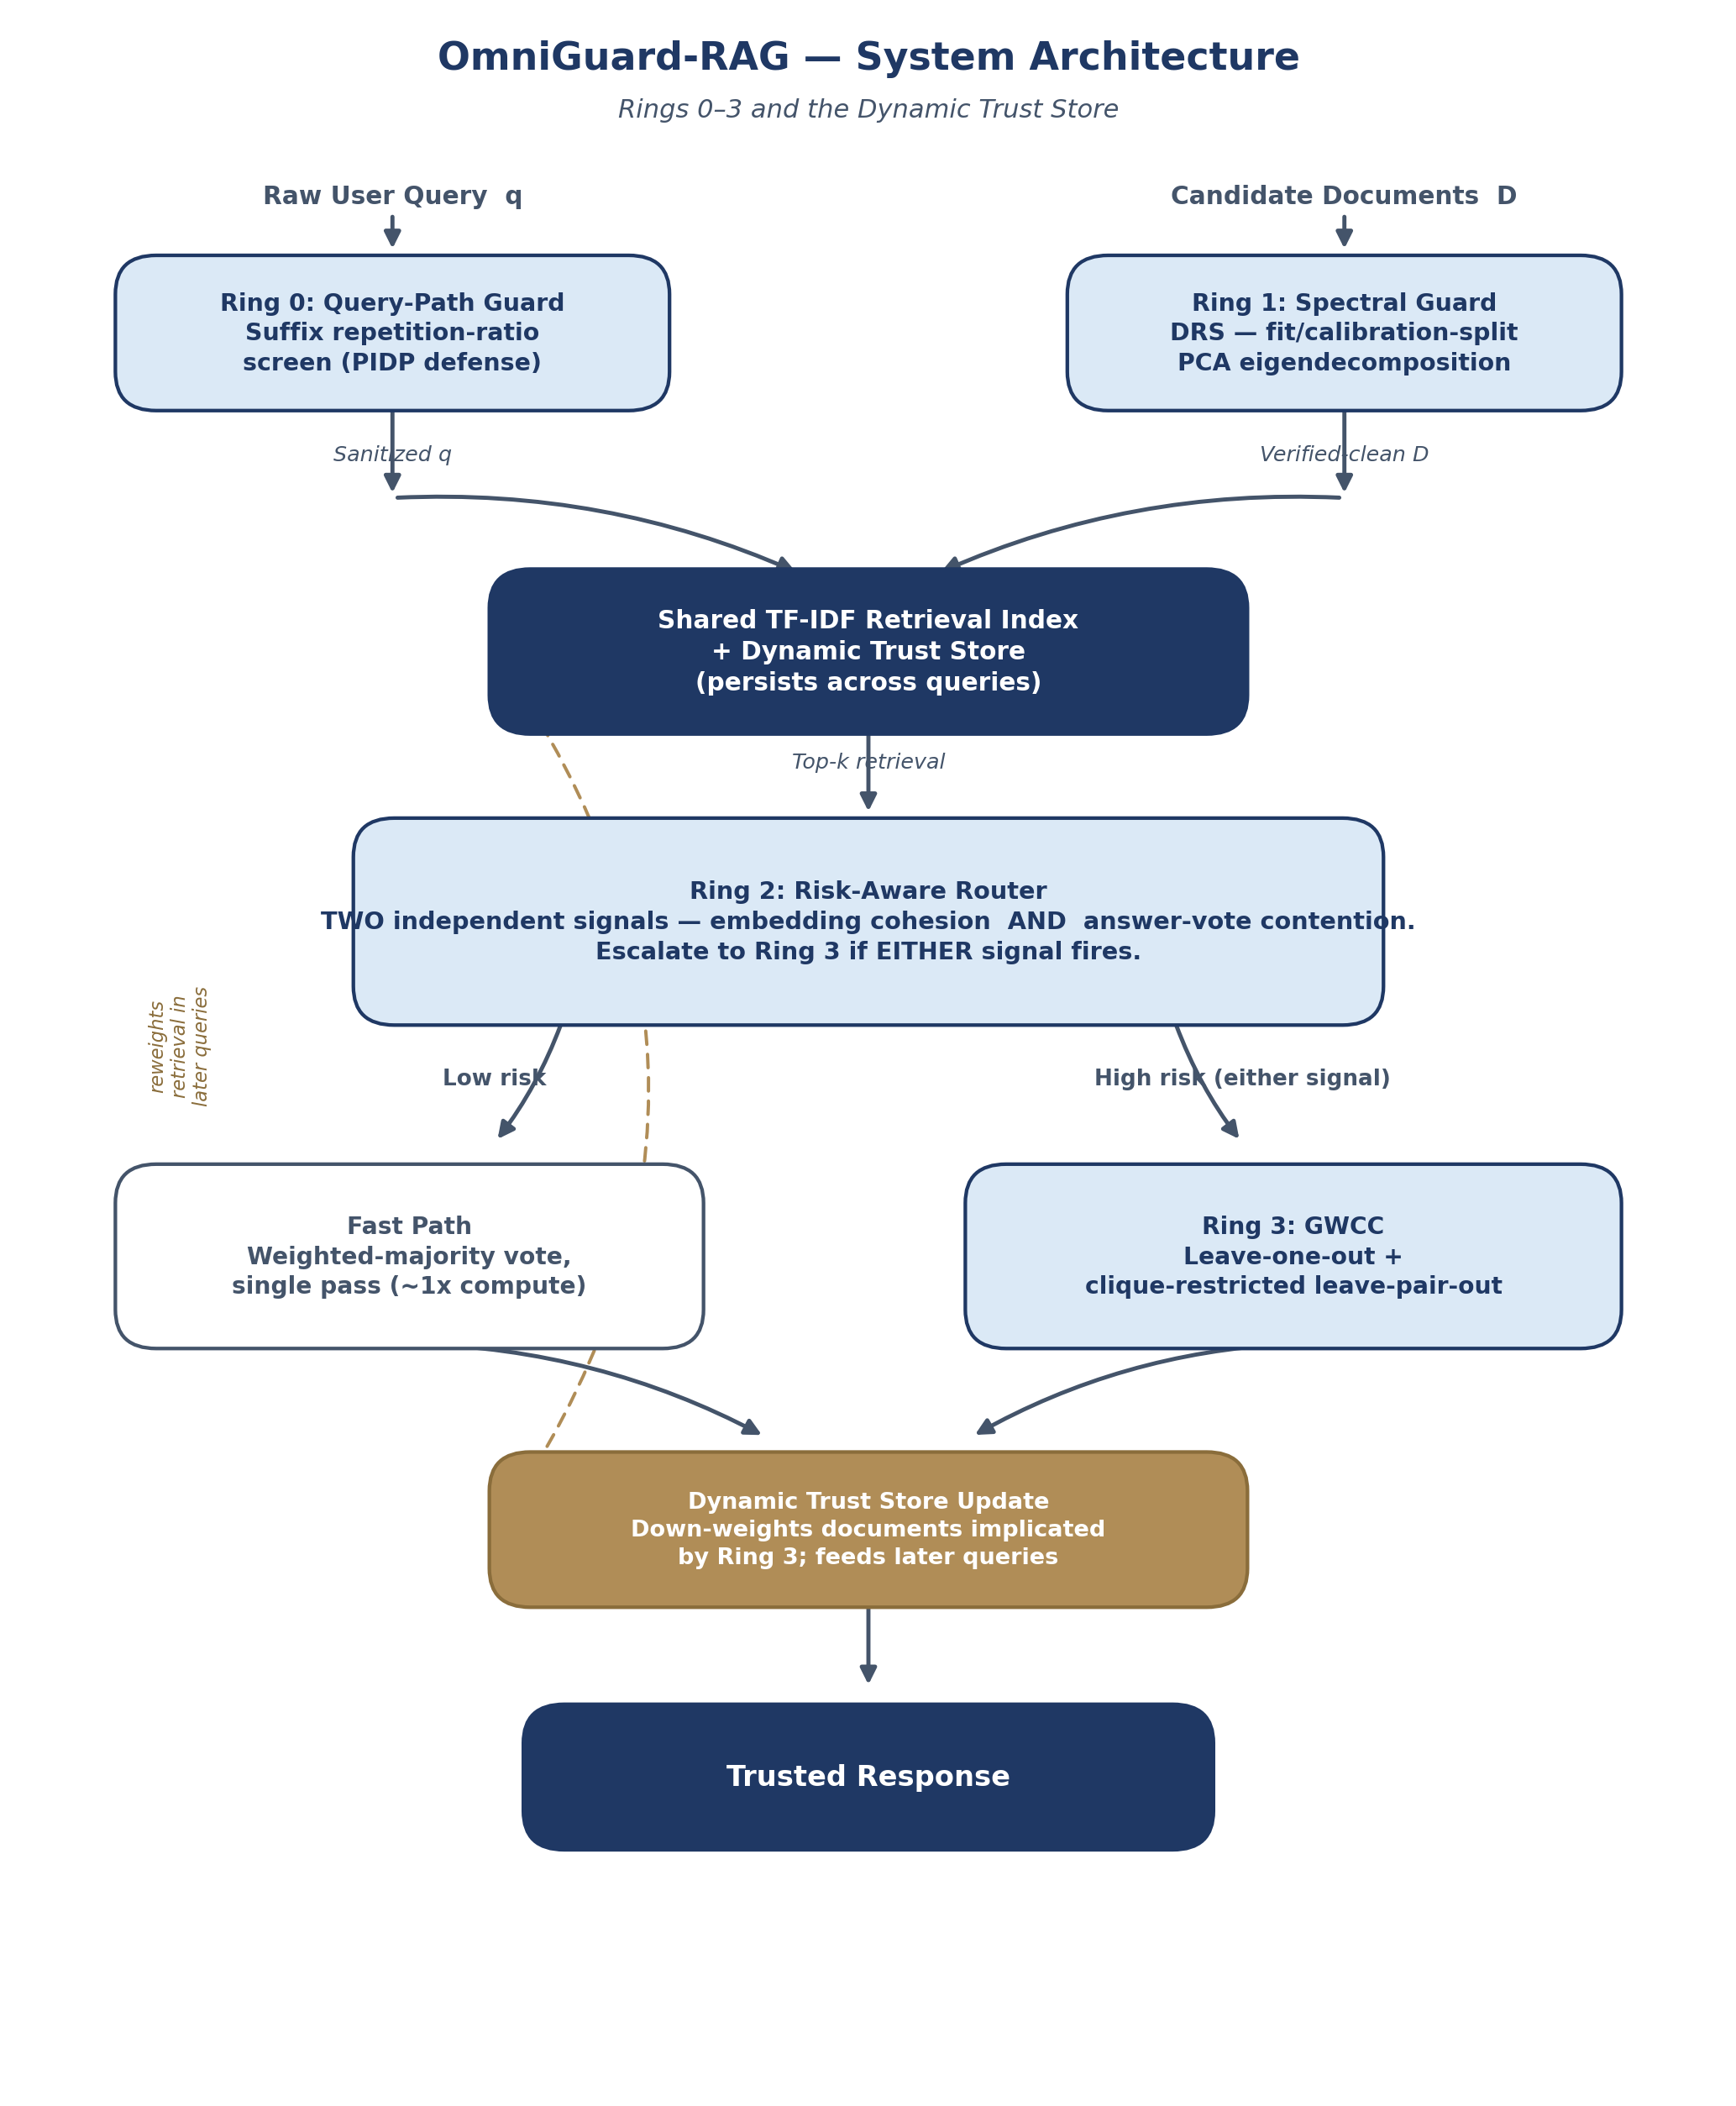
\includegraphics[width=0.72\textwidth]{figures/fig1_architecture.png}
\caption{OmniGuard-RAG system architecture --- Rings 0--3 and the Dynamic Trust Store.}
\label{fig:architecture}
\end{figure}

At a high level, the raw query and the candidate document pool are
screened independently and in parallel --- Ring~0 on the query, Ring~1 on
the corpus --- before either reaches the retriever. This independence
matters: a query-only or corpus-only defense is structurally blind to
whichever half of a compound attack it does not look at, which is
precisely PIDP's own design. The sanitized query and the DRS-verified
document pool then meet at a shared TF-IDF retrieval index, which also
applies the current Dynamic Trust Store weighting. Ring~2 evaluates the
resulting top-$k$ window and decides, per query, whether the fast path (a
single weighted-majority vote) is sufficient or whether the query must be
escalated to Ring~3's more expensive Group-Wise Counterfactual Consensus.
Whichever path answers the query, the Dynamic Trust Store is updated
afterward, so a document that behaved suspiciously in one query enters
the next query already down-weighted.

Module-to-ring mapping, for reference throughout the rest of this
section:

\begin{itemize}
\item \ringcode{query\_guard.py} --- Ring 0: query-path suffix guard
\item \ringcode{drs\_filter.py} --- Ring 1: spectral ingestion guard (fit/calibration-split PCA)
\item \ringcode{risk\_router.py} --- Ring 2: risk-aware router (cohesion + answer contention)
\item \ringcode{gwcc\_consensus.py} --- Ring 3: Group-Wise Counterfactual Consensus
\item \ringcode{omniguard\_pipeline.py} --- end-to-end orchestration and the Dynamic Trust Store
\item \ringcode{attack\_simulator.py} --- the six attack regimes evaluated in \Cref{sec:results}
\item \ringcode{baselines.py} --- the five reference-implementation baselines compared against
\item \ringcode{bench\_common.py, stats\_utils.py, ablations.py} --- shared evaluation plumbing, described in \Cref{sec:eval-methodology}
\end{itemize}

\subsection{Algorithms, Techniques, and Defense Mechanisms}

\subsubsection{Ring 0 --- Query-Path Guard (\ringcode{query\_guard.py})}

Ring~0 screens the incoming query text itself, before it is embedded, for
the token-repetition signature of a PIDP-style adversarial suffix. It
computes a repetition ratio over any candidate suffix --- the fraction of
tokens in that suffix that repeat a token already seen earlier in the
same span --- and strips the suffix if that ratio meets or exceeds a
threshold of 0.5 (i.e.\ at least half the suffix's tokens are repeats).
This threshold is a fixed, measured constant (\texttt{REPETITION\_THRESHOLD}
in \ringcode{query\_guard.py}) rather than a value tuned against attack
outcomes: keyword-stuffed injection suffixes are repetitive by
construction, since their entire purpose is to force specific tokens to
dominate the query's embedding, while genuine question text is not. Only
the sanitized query is passed forward to embedding and retrieval.

\subsubsection{Ring 1 --- Spectral Ingestion Guard: DRS (\ringcode{drs\_filter.py})}

Ring~1 implements Directional Relative Shifts directly: a real PCA
subspace, computed via NumPy SVD, fit on the TF-IDF vectors of a trusted
reference corpus. The lowest-variance directions of that subspace ---
where genuine clean documents barely move --- are kept, and any candidate
document whose whitened projection onto those directions exceeds a
calibrated threshold is dropped before it ever reaches the retriever.

The critical design choice, reached only after a serious self-referential
bug (\Cref{sec:debugging}, bug \#6) was found and fixed, is a
fit/calibration split: the reference corpus is partitioned into a fit
subset, which defines the low-variance subspace itself, and a held-out
calibration subset that never participates in the SVD fit and is used
only to set the rejection threshold. A brand-new, non-malicious document
is thereby scored exactly the way a calibration document was scored ---
never compared against its own defining sample.

\textbf{Parameters (measured constants in \ringcode{drs\_filter.py}):}
\texttt{LOW\_VARIANCE\_FRACTION = 0.4} (the lowest 40\% of variance-ranked
directions are retained as the detection subspace), \texttt{CALIBRATION\_FRACTION
= 0.3} (30\% of the reference corpus is held out for threshold
calibration and excluded from the SVD fit), \texttt{FILTER\_PERCENTILE =
99.0} (the rejection threshold is the 99th percentile of the calibration
split's own scores).

Targets: documents whose vocabulary or statistics fall outside the clean
distribution --- standard poisoning, the corpus half of PIDP, and plain
(non-camouflaged) collusion, all of which carry a genuine lexical tell.

\subsubsection{Ring 2 --- Risk-Aware Router (\ringcode{risk\_router.py})}
\label{sec:ring2}

Ring~2 computes two independent, unsupervised signals on the top-$k$
retrieved documents and escalates to Ring~3 if either fires --- an OR
gate, not a weighted blend, so that a strong signal on either axis alone
is sufficient.

\begin{description}[leftmargin=0pt,style=nextline,font=\bfseries\color{navy}]
\item[Signal A --- Embedding cohesion.] Mean pairwise cosine similarity
  among the top-$k$ retrieved embeddings. Genuine topical retrievals are
  geometrically consistent; anything that disturbs retrieval quality
  lowers this value. Threshold \texttt{RISK\_THRESHOLD = 0.55}, calibrated
  from measured clean-only top-5 retrievals, which were never observed
  below approximately 0.58 cohesion.
\item[Signal B --- Answer contention.] The weighted vote-mass fraction
  among the top-$k$ that disagrees with the plurality answer, using the
  same similarity$\times$trust weighting the final vote itself uses ---
  not a privileged ground-truth signal, but the identical proxy
  \texttt{weighted\_majority} already relies on for every system in this
  evaluation. Measured directly: clean-only top-5 retrievals show exactly
  0.0 contention, always, across every seed tested ($n{=}200$/seed),
  because every genuine document belonging to one topic asserts that
  topic's one real answer. Threshold \texttt{CONTENTION\_THRESHOLD = 0.15}
  --- chosen with headroom above that measured 0.0 clean-query floor,
  since even the smallest observed nonzero contention already indicates
  the retrieved set is not unanimous.
\end{description}

Signal B exists specifically because Signal A cannot see a particular
class of attack: a document engineered to be geometrically
indistinguishable from genuine content (\Cref{sec:literature}'s
SilentRetrieval-style camouflage) will not depress cohesion, by
construction. Measured directly in this project (\Cref{sec:discussion}):
mean top-5 cohesion under a fully camouflaged stealth-collusion attack is
0.70, statistically indistinguishable from the 0.70 measured on entirely
clean queries. Ring~2's second, independent signal is what actually
detects this class of attack --- not a refinement of the first signal,
but a genuinely different axis of measurement.

\subsubsection{Ring 3 --- Group-Wise Counterfactual Consensus / GWCC (\ringcode{gwcc\_consensus.py})}
\label{sec:ring3}

Ring~3 generalizes RAGuard/ZKIP's own single-document leave-one-out logic
--- ``does removing this document change the answer? If so, distrust it
and recompute'' --- to colluding pairs, without treating the
generalization as a simple vote across counterfactual subsets (a version
of this ring that did exactly that turned out to be a genuine, measured
no-op; see \Cref{sec:debugging}, bug \#7).

\begin{enumerate}
\item \textbf{Singleton pass}, identical to RAGuard/ZKIP: for each
  retrieved document, remove it alone and recompute the vote. If the
  answer changes, that document is implicated.
\item \textbf{Pair pass}, restricted to genuine self-corroborating
  cliques: for each candidate pair of documents, both must (a) share the
  same answer as each other, (b) hold that answer as a self-contained
  clique with no other retrieved document corroborating it, and (c)
  currently be part of the winning answer. Only a pair meeting all three
  conditions is tested by removing both together; if the answer changes,
  both are implicated.
\item \textbf{Final answer}: a plain weighted-majority vote over the
  retrieved set with every implicated document excluded.
\end{enumerate}

The clique restriction in step 2 is not a minor refinement --- an
earlier, looser version that implicated any pair whose joint removal
changed the vote was built, tested, and rejected, because it excluded
correct-but-numerically-scarce evidence just as often as it excluded
genuine poison pairs, and measurably \emph{raised} attack success rather
than lowering it. Coverage of the pair pass is bounded and probabilistic
(\texttt{MAX\_PAIR\_SAMPLES} limits how many candidate pairs are checked
per query, for tractability), which is stated here as an explicit, honest
limitation rather than a claim of exhaustive $k'{=}2$ detection.

\subsubsection{Dynamic Trust Store (\ringcode{omniguard\_pipeline.py})}
\label{sec:trust-store}

Persistent, per-document trust scores that carry across queries within a
session, decaying when Ring~3 implicates a document and growing when a
document repeatedly corroborates the winning answer. Trust score enters
the retrieval weighting as a multiplicative factor on cosine similarity,
so a document that behaved suspiciously in an earlier query is already
down-weighted the next time it competes for a retrieval slot --- a
capability that is, by construction, unavailable to any ring that
evaluates one query in isolation. \Cref{sec:results}'s headline results
make this ring's contribution explicit rather than folding it silently
into the rest of the pipeline (\Cref{sec:ablation-results},
\Cref{sec:discussion}).

\subsubsection{Attack Simulator (\ringcode{attack\_simulator.py})}
\label{sec:attack-simulator}

All six attack regimes reuse one shared sentence generator
(\ringcode{text\_gen.py}) also used for genuine clean text, so that clean
and attack text share identical structural diversity --- real topical
vocabulary and real factual content across sixteen topics, not a single
memorized template that a filter could key on by accident
(\Cref{sec:shared-generator} discusses a real early bug of exactly that
kind).

\begin{itemize}
\item \textbf{Clean} --- no attack; the corpus-only, unattacked control regime.
\item \textbf{Standard} --- keyword-stuffed poison asserting a novel, incorrect answer; carries a genuine lexical tell.
\item \textbf{PIDP} --- a repetitive query-suffix trigger paired with an attractor document cluster in the corpus that the sanitized-vs-unsanitized query would retrieve differently.
\item \textbf{Collusion} --- two to three poison documents corroborating the same false answer with novel, detectable vocabulary.
\item \textbf{Stealth collusion} --- true camouflage: the same clean-text generator, asserting the correct answer's own wording, with no lexical or spectral tell, additionally targeted to the specific keyword a given query names (Context-Adaptive Trigger Generation, after SilentRetrieval) so the poison genuinely competes for retrieval slots rather than being diluted by sheer corpus volume.
\item \textbf{Silent} --- a single camouflaged poison document, the stealth-collusion construction at $k{=}1$.
\end{itemize}

\subsection{Detailed Design Methodologies}
\label{sec:eval-methodology}

\subsubsection{Real text over synthetic vectors}

An early version of this project represented documents as abstract
Gaussian noise vectors carrying a hand-set ``evasion bias'' parameter ---
a design that let any target attack-success number be produced after the
fact simply by adjusting that parameter, which is the opposite of an
honest evaluation. The rebuild generates real, readable sentences from
real factual content across sixteen topics (photosynthesis, the TCP
handshake, the French Revolution, machine-learning overfitting, and
others), each with real keywords and real correct and incorrect answers,
embedded through a real, fixed scikit-learn \texttt{TfidfVectorizer}.
Whether a given attack survives a given filter is now an emergent
property of the actual generated text, not a parameter set directly.

\subsubsection{Shared generator for clean and attack text}
\label{sec:shared-generator}

A genuine early bug: clean documents were generated from one fixed
sentence skeleton, so Ring~1's spectral filter ended up keying on that
memorized boilerplate phrase rather than on topic content --- a filter
that happens to work is not the same as a filter that works for the
intended reason. The fix moved all sentence generation into one shared
module used by both clean and attack text, with five distinct sentence
templates. What is genuinely low-variance in the resulting corpus is
topic vocabulary itself, not one memorized string.

\subsubsection{Multi-seed statistical evaluation (\ringcode{bench\_common.py}, \ringcode{stats\_utils.py})}
\label{sec:multiseed}

\ringcode{bench\_common.py} centralizes world-building, the
attack-regime/scenario logic, and the timed per-system query loop in
exactly one place, imported by every benchmark entry point --- the
single-seed script, the ablation ladder, and the multi-seed evaluation
--- specifically so that a fix or a new regime added in one script cannot
silently fail to propagate to the others. \ringcode{run\_full\_evaluation.py}
runs eight independently regenerated corpora, query sets, and DRS
calibration splits (seeds 7, 11, 23, 41, 59, 79, 97, 113; not reshuffles
of one shared dataset), 200 queries each, 1,600 queries per system in
total, and \ringcode{stats\_utils.py} aggregates every metric as a mean and
a Student's-$t$ 95\% confidence-interval half-width rather than a bare
mean. Student's-$t$, not the more familiar $z=1.96$ normal-distribution
shortcut, is the textbook-correct choice for a small-sample mean with
unknown population variance --- exactly the regime an eight-seed
evaluation sits in --- and the single-seed edge case (zero degrees of
freedom) is reported as a bare point estimate with a zero-width interval
rather than a fabricated one.

\subsubsection{Held-out calibration discipline}

Every threshold in the pipeline is calibrated on data held out from
whatever it is being used to judge: Ring~1's rejection threshold comes
from a calibration split excluded from its own PCA fit; Ring~2's cohesion
and contention thresholds come from clean-only statistics measured on
fresh queries the router is not currently routing; Ring~0's repetition
threshold comes from clean-query statistics. This discipline exists
specifically because its absence caused the project's most serious bug
(\Cref{sec:debugging}, bug \#6): a filter fit and calibrated on the same
reference points will reject almost anything unfamiliar, which produces
an artificially perfect attack-success number that reflects
self-reference, not detection.

\subsubsection{Reproducibility}

All random processes in the evaluation use explicit, deterministic
seeds. One further fix was required for genuine reproducibility:
Python's built-in string \texttt{hash()} is randomized per process by
default, and an early version of the regime-selection logic depended on
it, so identical code and identical arguments produced different numbers
on two separate runs of the same script. Regime-name-derived seeds are
now mapped through a fixed integer table instead.

\subsubsection{Honest cost accounting}

Every system in this evaluation reports both an LLM-call-count estimate
and a real, measured wall-clock orchestration latency, because
\Cref{sec:compute-cost} shows the two rankings do not agree --- a system
with a low call count is not automatically the cheapest system to run,
and reporting only one of the two numbers would hide that.
